\chapter{Quality Assurance}
This chapter will cover the overall effort of the project to ensure a quality result. This involved automated testing, manual testing, and utilising adequate coding standards to ensure good maintainability.

\section{Overall Approach to Testing}
The overall approach with testing should revolve around ensuring all main features are tested, it is understood that some features are less testable than others, but a best effort attempt must be made to this effect. Most of the program should be tested, so that when a developer changes something or uses something that is not available in earlier APIs it shows up during testing, this was invaluable whilst attempting to ensure that the application works between the all versions of Android it is aimed at, 21+.

\section{Automated Testing}

Ensuring that any change to your code base, that causes a regression in application functionality is sometimes crucial in tracking down exactly what code causes the error, as a stack trace may not be enough. To achieve automated testing it is possible to cause Android Studio to test a target which includes Instrumentation, and Unit tests, whenever a code change is made, this disadvantageous on anything but the most basic project because it will not only take a long time up to 10 minutes per change, but also slow your computer down. 

Bitrise is the solution, it is a cloud based free to open source projects platform specialised in phone development and testing for Android and iOS. It is discussed in detail earlier in the report in Section \ref{CI}. What was looked for in a Continuous Integration solution, was an easy to use, expandable and ability to test not only unit tests, but UI Integration tests on every single API, and language the application supports. Bitrise fits all of the requirements for a Continuous Integration platform set forth in this section, as long as the project is open-source, which it is.

The Automated tests are completed on Bitrise and for the repository can be shown with a green tick as all tests are passing that are conducted automatically, shown in Figure \ref{fig:bitriseBuilds}.

 \begin{figure} [htbp!]
        \centering
        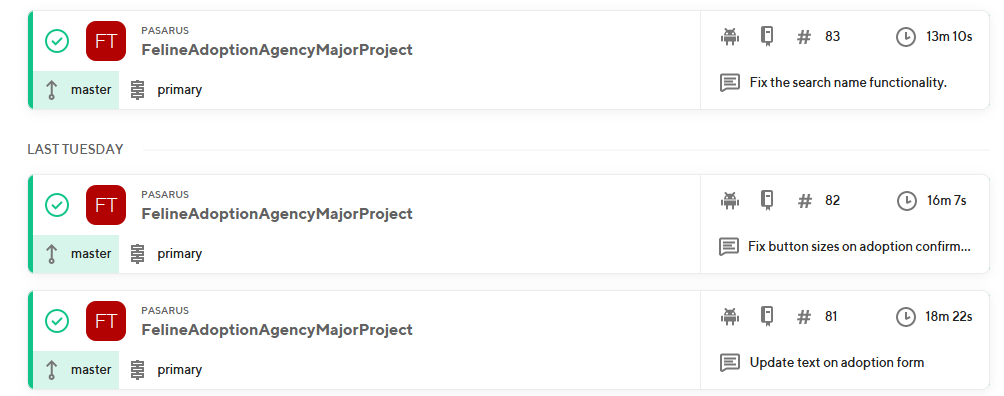
\includegraphics[width=\textwidth]{Images/Bitrise Repo Builds.PNG}
        \caption{The 3 most recent builds of the repository on Bitrise}
        \label{fig:bitriseBuilds}
    \end{figure}

\section{Test Implementations}

This project had a heavy emphasis on testing, where possible tests were implemented quickly and effectively. In some areas of the code base there is no testing, this revolves around the requirement for a user to log in, the main aim, was to provide testing not only on the Continuous Integration platform but locally, getting a Firebase Authenticated User and local Firebase database seemed challenging and thus was pushed to a later sprint, for when development of key user features had been completed, this was not possible given time constraints. Currently there is a lack of testing on any feature revolving around a user logging in, so manual testing must step in to fill this void.

The project implements 3 main areas of testing, manual testing, unit tests and user interface integration testing, the latter 2 of which is performed on every iteration of the code base that is committed to the GitHub repository.

    \subsection{Unit Tests}
    Unit Tests are currently in use for 2 files 1 class and 1 utilities file, this is because these are the parts of the system that can be tested without UI elements present. Meaning that the functionality and operation does not partially or completely require a Android Activity to be present in order to operate functionally. If a class or function is implemented separately from a Fragment or Activity. Every aspect of the classes and functions that are implemented should be tested to ensure guaranteed functionality, therefore every branch of code execution should be tested during testing with Unit Tests, this should be very possible and the test example shows this in Appendix Section \ref{Unit Test Example}. The Unit tests are ran on both Debug and Release testing sets during Continuous Integration builds, the completed tests on Bitrise are shown in Figure \ref{fig:UnitTestsStatus}.
    
    \begin{figure} [htbp!]
        \centering
        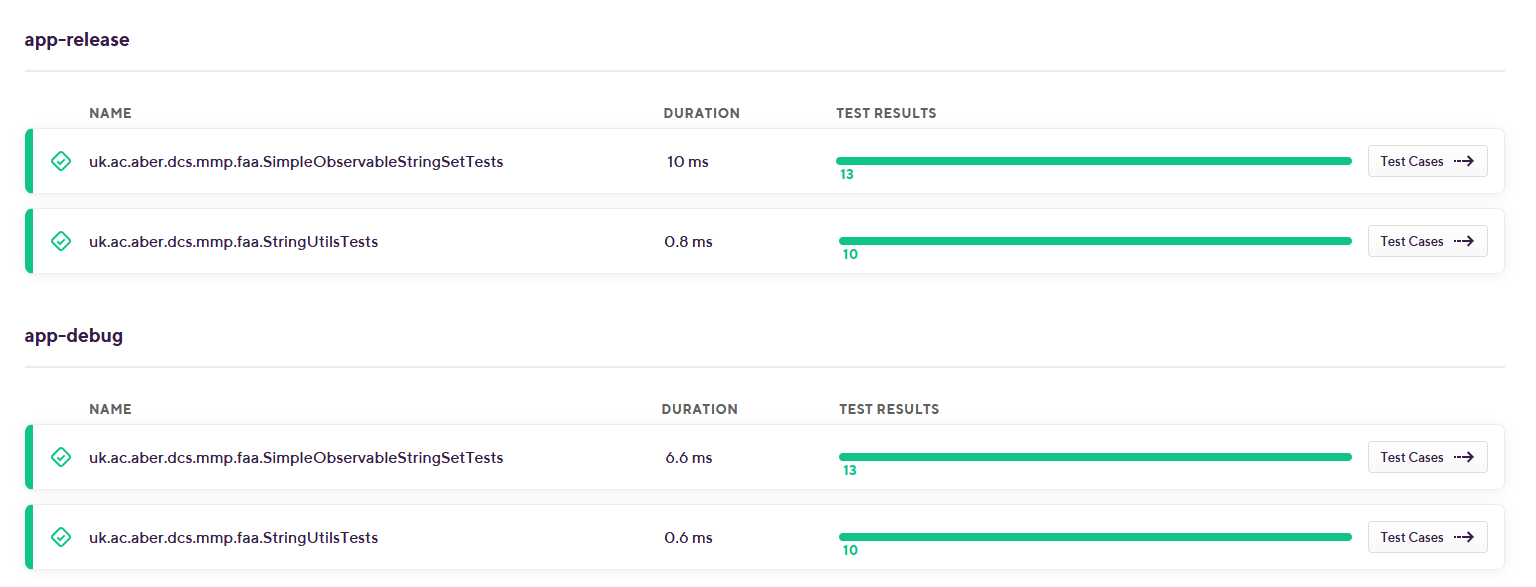
\includegraphics[width=\textwidth]{Images/UnitTestsBitrise.PNG}
        \caption{Unit Tests completion on most recent Bitrise Build}
        \label{fig:UnitTestsStatus}
    \end{figure}
    
    \subsection{User Interface Integration Testing}
    The project makes heavy use of UI Instrumentation tests in the form of Integration tests. Currently the project tests every UI aspect, to test that it is appearing correctly, with the exception of anything locked behind the Authentication methodology. The integration tests have the added benefit that they ensure that the application opens and all the tests can be ran on every API 21 and above, specifically via the usage of the Continuous Integration platform. The completed Bitrise UI Instrumentation Integration tests are shown to be completed in the Figure \ref{fig:UIIntegrationTests}.
    
    \begin{figure} [htbp!]
        \centering
        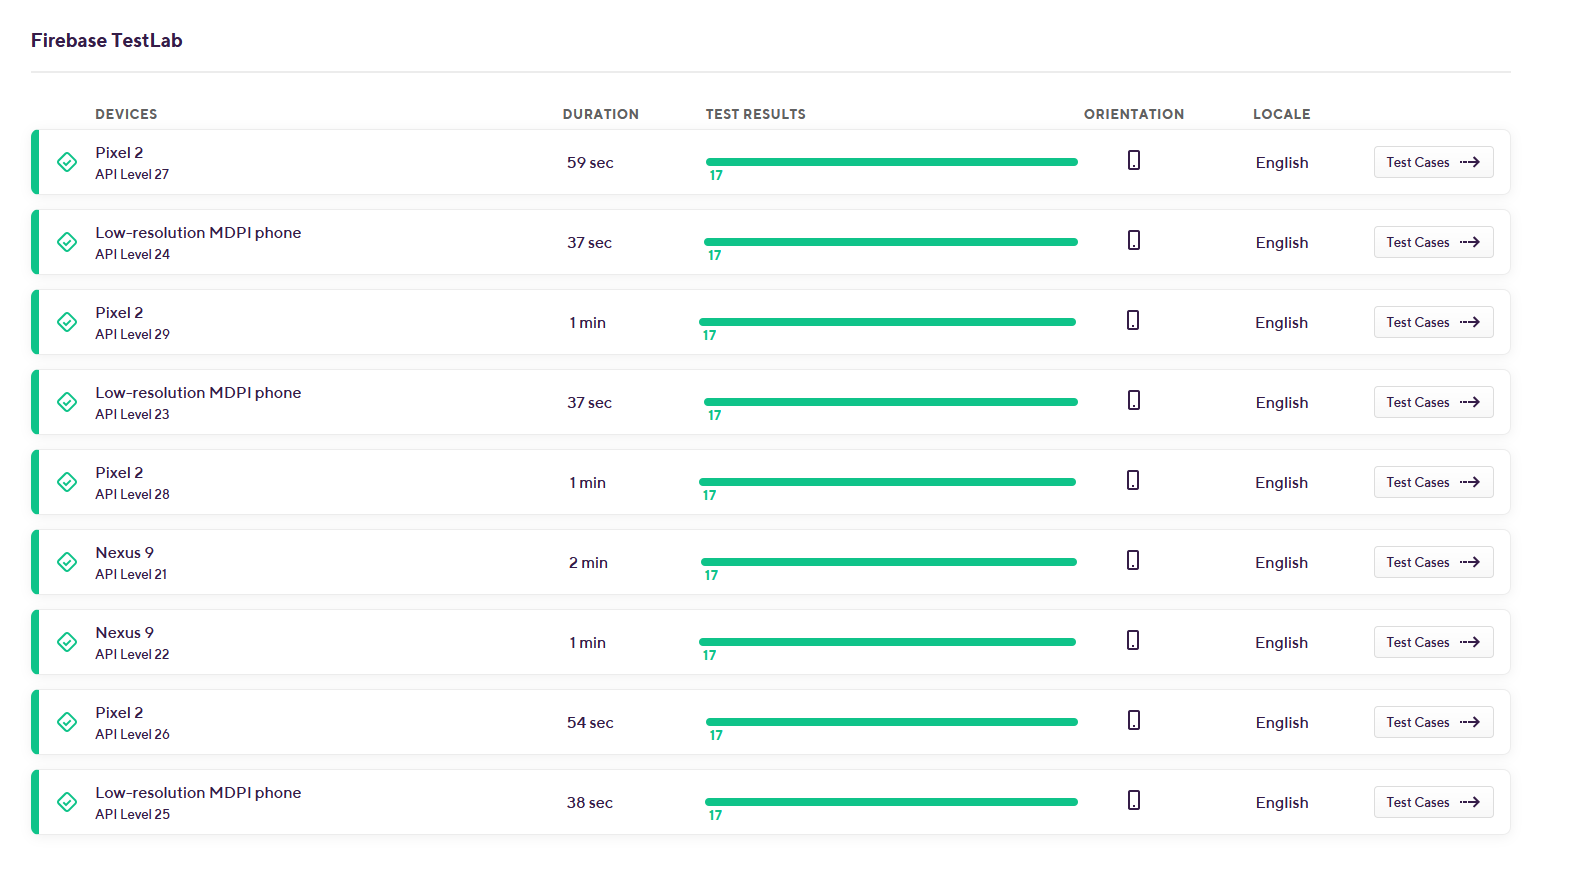
\includegraphics[width=\textwidth]{Images/UI Integration Tests Bitrise.PNG}
        \caption{UI Instrumentation Integration tests completion on most recent Bitrise Build}
        \label{fig:UIIntegrationTests}
    \end{figure}
    
    Each test is intended to be created using the Espresso test recorder, tested locally, ensuring that database connections are waited for correctly, and then pushed to the GitHub Repository, and monitored, if the tests fail a fix should be created and tested in the cycle again. These tests were absolutely instrumental in the development of the application as it lead to the discovery and fix of many high level UI and Application wide bugs, this echos the benefits of the tests.
    \clearpage

    \subsection{Manual Testing}
    Due to the lack of coverage of the Authentication features. The nature of manual testing ensures that the tester looks at most of the application and tries to find areas that have not worked well or are currently not fully functional. A Manual Testing table has been created to ensure that certain features are functional/present it is view-able on table \ref{tab:MANUALTESTINGSERVER}.

\footnotesize \small
\begin{longtable}{|l|l|l|l|l|}
\hline
\textbf{} &
  \textbf{Test Case Description} &
  \textbf{Test Steps} &
  \textbf{Expected Result} &
  \textbf{Pass/Fail} \\ \hline
\endhead
%
\#1 &
  \begin{tabular}[c]{@{}l@{}}Ensure login functionality\\  works\end{tabular} &
  \begin{tabular}[c]{@{}l@{}}1) Open application\\ 2) Tap navigation draw \\ button\\ 3) Tap login\\ 4) Select email\\ 5) Enter email\\ 6) Enter password\end{tabular} &
  \begin{tabular}[c]{@{}l@{}}1) User successfully logged in\\ 2) Adoption statuses should be \\ updated\\ 3) Nav draw login button\\  replaced with My Account \\ button\\ 4) Saved cats are shown on the\\  Saved Cats tab\end{tabular} &
  Pass \\ \hline
\#2 &
  \begin{tabular}[c]{@{}l@{}}Ensure Feedback \\ functionality works\end{tabular} &
  \begin{tabular}[c]{@{}l@{}}1) Login using test case \#1\\ 2) Tap nav draw\\ 3) Tap feedback\\ 4) Enter Feedback details \\ into feedback text box\\ 5) Tick the box to ask \\ to be replied to by the \\ developer\\ 6) Tap Send\end{tabular} &
  \begin{tabular}[c]{@{}l@{}}1) Feedback appears in the \\ Firebase Firestore feedback\\ collection under the logged in\\ User's UID and date.\end{tabular} &
  Pass \\ \hline
\#3 &
  \begin{tabular}[c]{@{}l@{}}Ensure user data is \\ synced across devices\end{tabular} &
  \begin{tabular}[c]{@{}l@{}}1) Login using test case \#1\\ 2) Tap nav draw\\ 3) Tap My Account\\ 4) Add or change the text\\  fields under the adoption\\  status and tap update.\\ 5) Tap logout\\ 6) Login again using \\ test case \#1\\ 7) Tap Nav Draw\\ 8) Tap My Account\end{tabular} &
  \begin{tabular}[c]{@{}l@{}}1) All changed or added text\\ should be loaded back into the\\ text fields.\end{tabular} &
  Pass \\ \hline
\#4 &
  \begin{tabular}[c]{@{}l@{}}Ensure saving cats\\  syncs across login\\  sessions and devices\end{tabular} &
  \begin{tabular}[c]{@{}l@{}}1) Login using test case \#1\\ 2) Tap the cat finder \\ button on Bottom \\ Navigation Bar\\ 3) Tap the heart icon on \\ a few Cat Cards\\ 4) Tap nav draw\\ 5) Tap My Account\\ 6) Tap Logout at the \\ bottom of the scroll\\ 7) Login again using\\  test case \#1\\ 8) Tap the saved cat \\ button on\end{tabular} &
  \begin{tabular}[c]{@{}l@{}}1) The cats that were saved\\  should appear on the screen\end{tabular} &
  Pass \\ \hline
\#5 &
  Adoption is functional &
  \begin{tabular}[c]{@{}l@{}}1) Login using test case \#1\\ 2) Tap the cat finder\\ button on Bottom\\ Navigation Bar\\ 3) Select a Cat Card\\ 4) Scroll to bottom\\ 5) Click Adopt This Cat!\\ 6) Fill/change data and tap \\ update\\ 7) Tap Yes\end{tabular} &
  \begin{tabular}[c]{@{}l@{}}1) Ensure that cat has appeared\\ in the adoption statuses\\ 2) Navigate to My Account and\\ ensure that the updated data is\\ present\end{tabular} &
  Pass \\ \hline
\#6 &
  Dark Mode is functional &
  \begin{tabular}[c]{@{}l@{}}1) Tap settings icon\\ 2) Flip Dark Mode switch\\ to on\\ 3) Tap the Up Button\\ 4) Tap the featured cat\\ 5) Tap the Up Button\\ 6) Tap each button on the\\ Bottom Navigation Bar\\ 7) Tap nav draw\\ 8) Navigate to each nav \\ draw location and then \\ back up to home before\\ continuing to the next\\ location, including\\ Settings, About, Login,\\ Help, and Feedback.\\ 9) Login using test case \#1\\ 10) Tap nav draw\\ 11) Tap My Account\\ 12) Tap an adoption status\\ card if present otherwise,\\ adopt a cat then come \\ back.\end{tabular} &
  \begin{tabular}[c]{@{}l@{}}1) Each of the screens should\\ look like the dark mode theme\\ is being used.\end{tabular} &
  Pass \\ \hline
\caption{Manual Testing table}
\label{tab:MANUALTESTINGSERVER}\\
\end{longtable}

\footnotesize \normalsize

\section{Coding Standards and Maintenance}

Using good coding standards makes code more readable and easier to maintain. For example, if a file contains multiple ways of defining a variable it can become harder to read and rather distracting. Enforcing a good use of comments and public API documentation allows a developer to understand how a class functions without ever looking at the code in the first place, this allows for quicker and easier maintenance and future development.

The Coding Standards in place on this project for Kotlin are provided on the Kotlin website \cite{KOTLINCODINGSTANDARDS}. It's a set of guidelines and helpful tips for easier to read Kotlin, if every developer on the team follows these standards it allows developers to read the code much faster and get less distracted.

Python also is used in the project specifically in the server scripts (Section \ref{SERVERSCRIPTS}) for Python the universal developer standards rest up on using the PEP8 standards \cite{PEP8STANDARDS}. The PEP8 standards are enforced by PyCharm, the IDE used during this project for Python development. 

